\chapter{Trabajos Relacionados}

En el presente capítulo comenzaremos discutiendo sobre un trabajo que optimiza un \emph{splitter}.
Seguidamente, identificaremos dos inconvenientes con este trabajo e iremos mostrando como otras 
investigaciones han afrontado estos desafíos.

En \cite{Prosopio-Galarza2019} se optimizó un \emph{splitter} con guías de onda fijas de $0.5 \mu m$, 
donde las guías de onda de salida son separadas por $0.2 \mu m$ y 
todas estas son unidas con una región rectangular de diseño de $2 \mu m \times 1.5 \mu m$.
Con esta geometría se simulan distintos diseños dividiendo la región rectangular en ($z = 13$) segmentos
uniformemente separados.
Cada segmento puede variar su altura dentro del rectángulo, estos se centran de forma vertical y
se van uniendo sus extremos. 
La representación de esta idea la podemos observar en la \autoref{fig:roy-mmi} con $z = 5$ segmentos.

\begin{figure}[ht]
  \centering
  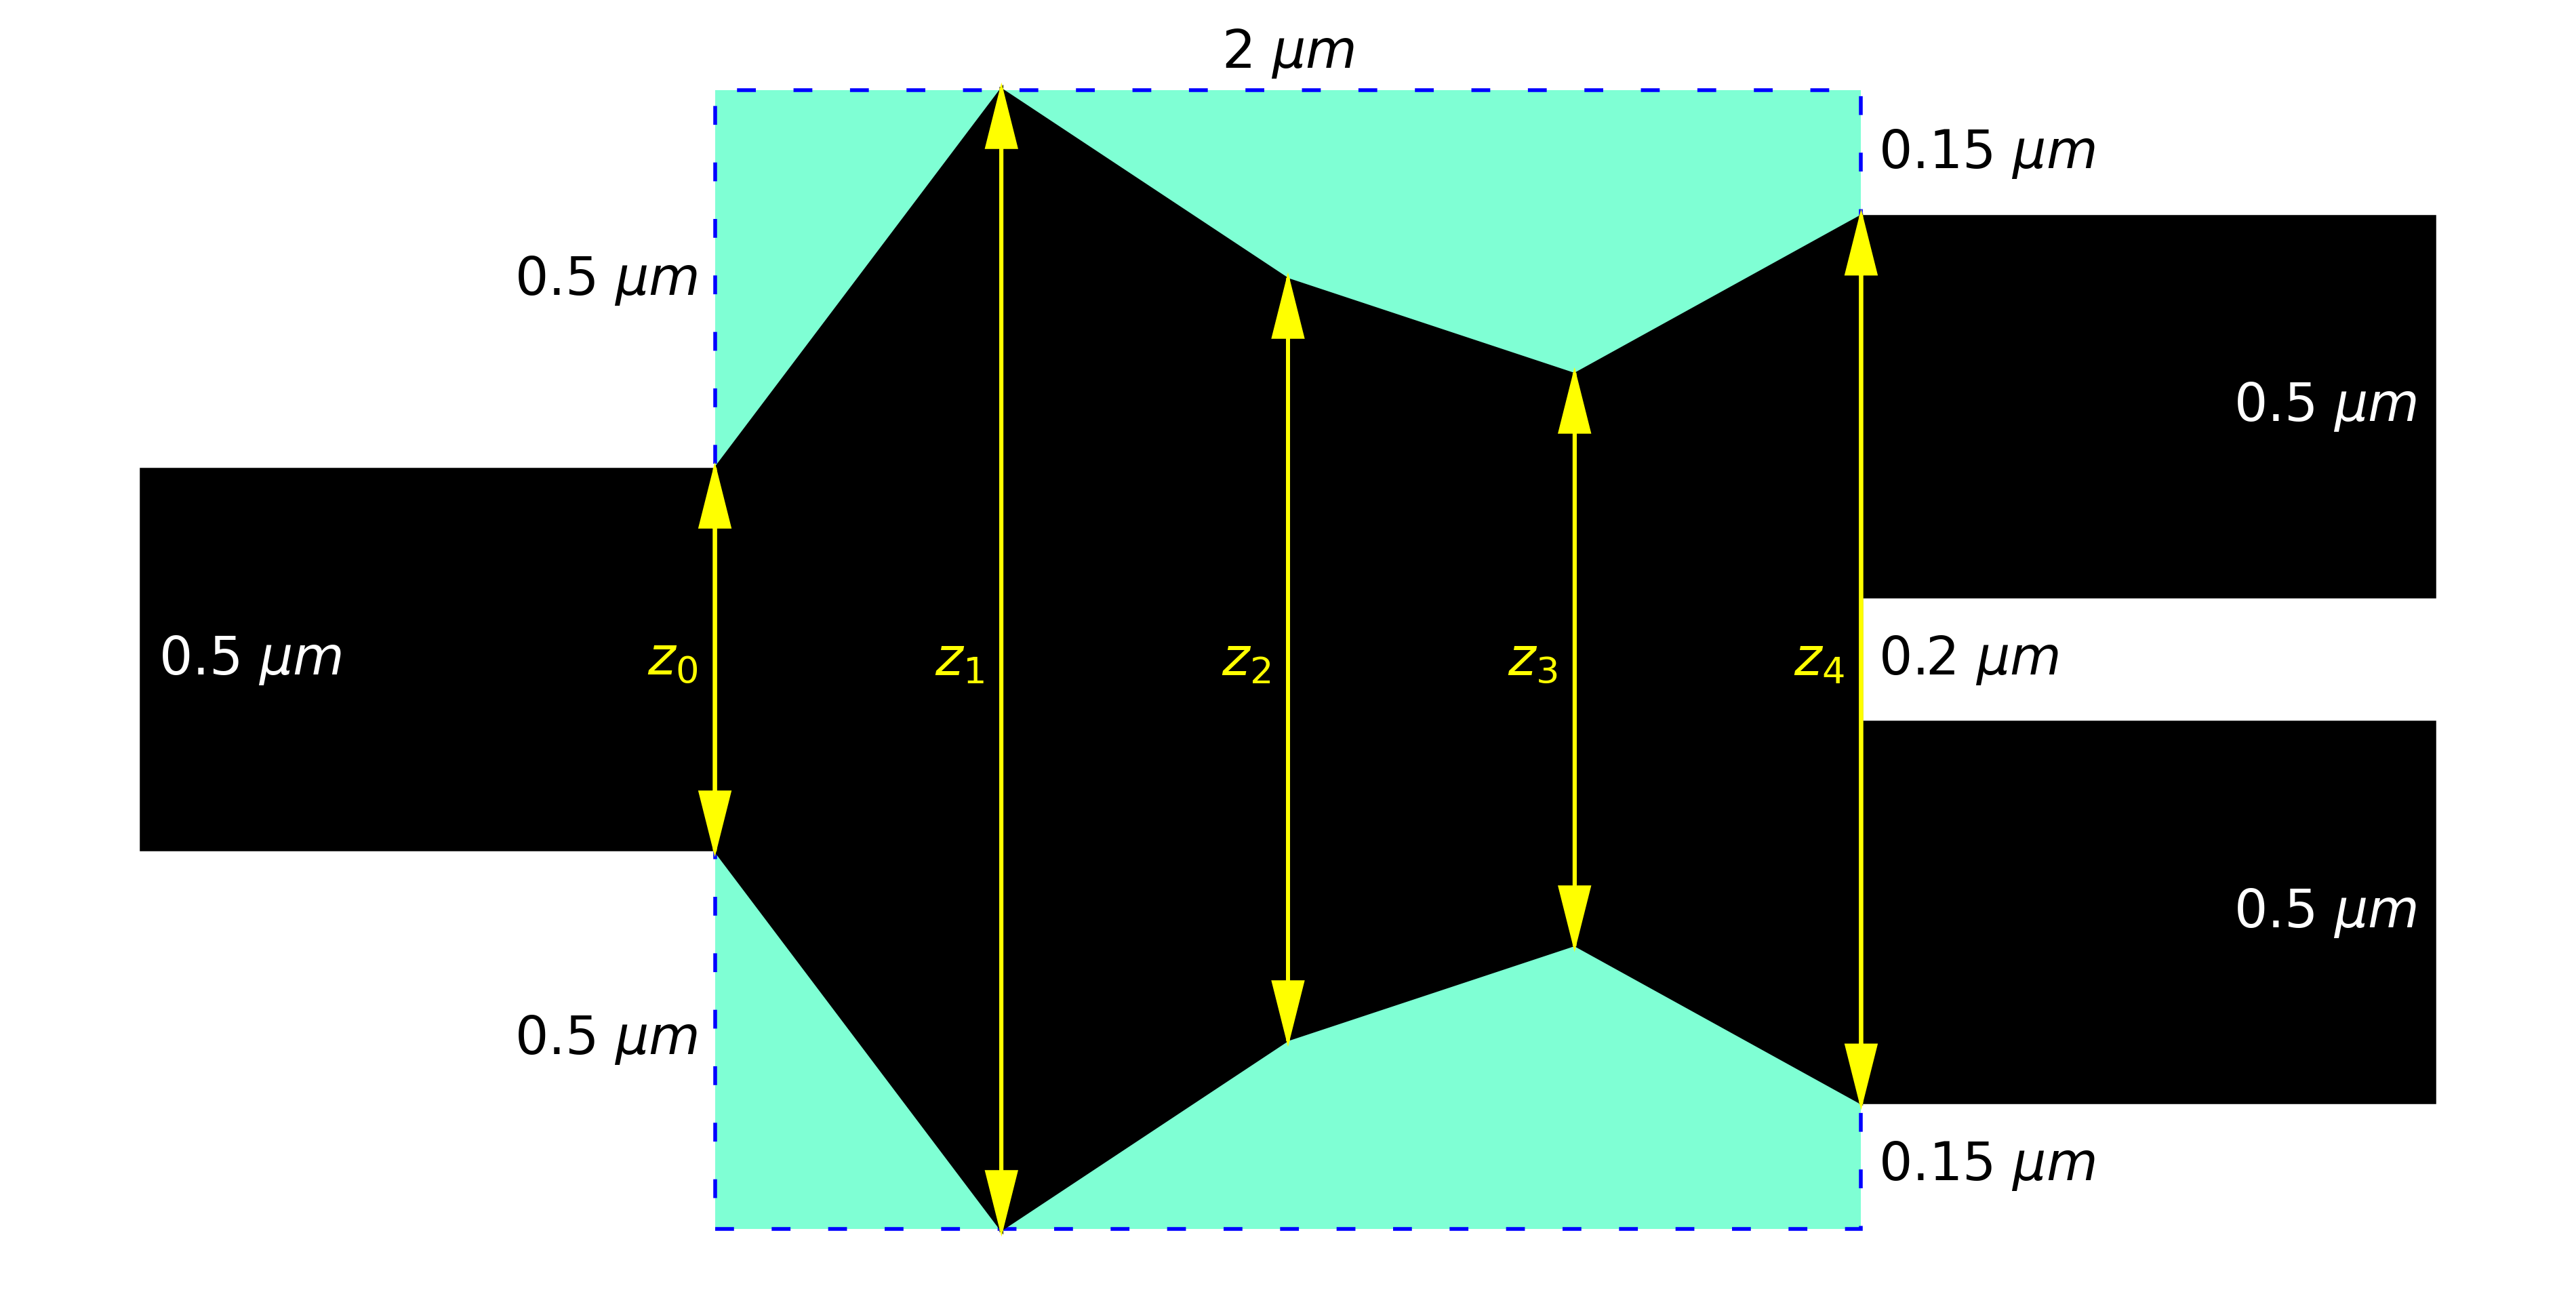
\includegraphics[scale=0.5]{image/related-works/mmi-angles.png}
  \caption{Diseño de un \emph{splitter} basado en \citep{Prosopio-Galarza2019} utilizando $z = 5$ segmentos.} 
  \label{fig:roy-mmi}
\end{figure}

Como función objetivo se establece maximizar la transmitancia en la guía de onda superior trabajando con una
longitud de onda de $1550 nm$.
Los mejores resultados son obtenidos al usar PSO como algoritmo de optimización.

Es destacable que al usar esta parametrización se puede limitar las alturas de los segmentos para asegurar 
obtener ángulos agudos, los cuales son los más adecuados como regla práctica de diseño
\citep{LukasChrostowski2010}.
Sin embargo, hay dos inconvenientes con este trabajo:

\begin{itemize}
  \item \textbf{Inconveniente 1:} 
  La parametrización utilizada descarta la posibilidad de diseños menos 
  intuitivos (por ejemplo, con agujeros) que podrían ocupar menor área y mantener una buena transmitancia.
  
  \item \textbf{Inconveniente 2:}
  Las optimizaciones solo se repitieron una vez con apenas 30 iteraciones y una población de 14 individuos.

\end{itemize}


A continuación, vamos a desarrollar en más detalle como otros trabajos han buscado solucionar estos dos inconvenientes.

\section{Inconveniente 1: La Parametrización}

Como se detalla en \cite{Molesky2018}, para permitir diseños con mayor grado de libertad se suele 
trabajar con dos enfoques:
(i) parametrización basada en conjuntos de nivel y
(ii) parametrización basada en píxeles.


La parametrización basada en conjuntos de nivel permite describir geometrías poco intuitivas,
con elevada transmitancia y sin necesidad de regiones grises.
\cite{Piggott2015} utiliza esta parametrización para optimizar un WDM con guías de onda de $0.5 \mu m$
y una región de diseño de $2.8 \mu m \times 2.8 \mu m$ trabajando a $1300 nm$ y $1550 nm$.
Comienza con un diseño inicial aleatorio, luego realiza la optimización en tres etapas consecutivas:
(i) optimiza sin restricciones con una parametrización basada en píxeles (pudiendo producir regiones grises),
(ii) introduce una parametrización basada en conjuntos de nivel,
(iii) busca optimizar en distintas longitudes de onda con el fin de buscar un diseño robusto.
Este enfoque ha dado buenos resultados incluso al fabricarse. 
Además, en \cite{Piggott2017} se desarrolla
un algoritmo para tratar de imponer un mínimo radio de curvatura a los diseños y asegurar 
mayor coherencia entre las simulaciones y los diseños fabricados.

De manera similar, \cite{Su2020} obtiene transmitancias alrededor de $90\%$ al
optimizar un WDM trabajando a $1400nm$ y $1550 nm$.
Sin embargo, su proceso de optimización consiste en solo dos etapas:
(i) optimización continua y
(ii) optimización discreta.
Lo interesante de su propuesta es que en la optimización continua trabaja con subetapas donde aplica
una transformación sigmoidal (similar a la \autoref{eq:projection}) para ir discretizando los diseños.
Luego, en la optimización discreta aplica una parametrización basada en conjuntos de nivel para 
eliminar regiones grises e imponer un mínimo radio de curvatura de $100 nm$.


Por otro lado, la parametrización basada en píxeles también ha obtenido buenos resultados en
la optimización topológica.
Como se describe en \cite{Lazarov2016}, generalmente se utiliza las transformaciones 
descritas en la \autoref{sec:transformations}:
filtro por densidad y proyección. Particularmente, utilizando estas mismas transformaciones
se logra simular dos posibles errores de fabricación: dilatación y erosión.
A modo de tutorial, \cite{Christiansen2021} optimiza un WDM con guías de onda de $0.299 \mu m$ y
una región de diseño de $2 \mu m \times 2 \mu m$ trabajando a $1300 nm$ y $1550 nm$.
Utilizando parametrización basada en píxeles, 
realiza un proceso similar a la optimización continua de \cite{Su2020}; 
pero, en vez de aplicar una función sigmoidal para 
discretizar el diseño, aplica el filtro por densidad para tratar de imponer un mínimo radio de curvatura
y después la proyección para discretizar los diseños. 
Asimismo, define su función objetivo de tal modo que asegura
diseños robustos ante dilatación o erosión.


De manera similar \cite{Hammond20} trabaja con optimización topológica robusta para optimizar un 
\emph{splitter} en una región de diseño de $3 \mu m \times 3 \mu m$.
En este trabajo se realiza la optimización imponiendo distintos radios de curvatura.
De sus resultados se puede observar que a menor radio de curvatura se logra definir más detalles en los
diseños y la optimización logra mejores resultados.
Posteriormente, \cite{Hammond21} fabrica diseños obtenidos con esta idea y muestra buenos resultados. 
Pero, detallan la presencia de pequeñas variaciones en las simulaciones y datos experimentales
posiblemente causada por regiones aisladas en el diseño.

\section{Inconveniente 2: La Optimización}

En \cite{Malheiros-Silveira2020} se compararon dos algoritmos en la optimización de un dispositivo.
A diferencia de \cite{Prosopio-Galarza2019}, la comparación no se realizó en base a la cantidad de iteraciones
realizadas por cada algoritmo, en cambio se hizo de acuerdo a la cantidad de simulaciones realizadas 
($\approx 2000$), es decir, la cantidad de veces que se evaluó la FOM.
Esta estrategia es más adecuada para comparar algoritmos con distintas características de una manera más justa.


En otros trabajos que se centran en comparar algoritmos para optimizar un mismo dispositivo se sigue la misma
idea para la comparación \citep{Schneider2019, Gregory2015}; sin embargo, no parece haber un consenso sobre algún algoritmo que funcione bien
para optimizar cualquier dispositivo.


En general, PSO y GA han sido extensamente usados en el área de acuerdo de acuerdo a reseñas como las de
\cite{Elsawy2020} y \cite{Campbell2019}. Tal y como es señalado en estos trabajos, el desempeño de ambos
algoritmos es sensible a los parámetros escogidos. Este es un gran inconveniente debido a que escoger
parámetros adecuados puede consumir mucho tiempo y esto se debe hacer independientemente para cada
dispositivo. Con el propósito de superar esta dificultad, distintos trabajos están optando por usar algoritmos
que no necesiten configurar parámetros internos.


Bajo este enfoque, en \cite{Gregory2015} se resaltó el buen desempeño que pude obtener el algoritmo CMA-ES en
la optimización de ciertos dispositivos, llegando a superar al PSO.
De manera similar, en \cite{Schneider2019} se realizó un trabajo muy completo comparando distintos algoritmos
llegando a resultados donde la optimización bayesiana mostró los resultados más prometedores,
pero esta comparación fue para un bajo número de parámetros ($< 15$).
Y, aunque no detalla la razón, en \cite{Su2020} se empleó el algoritmo 
L-BFGS-B en la optimización de un \emph{bend} y WDM llegando a obtener resultados destacados.

Un aspecto importante a resaltar de estos últimos tres trabajos es que al comparar distintos algoritmos para
optimizar dispositivos fotónicos necesitamos contar con
(i) un elevado número de simulaciones y
(ii) distintas ejecuciones que comiencen con diferentes puntos iniciales.

Como se ha discutido en este capítulo, la parametrización de nuestros dispositivos usando un bajo número
de parámetros puede ir condicionando nuestros resultados, ante ellos dos posibles soluciones son usar
(i) parametrización basada en conjuntos de nivel o (ii) parametrización basada en píxeles. 
Esto supone nuevos desafíos, mas ya existen estrategias para afrontarlos e
incluso para incluir restricciones de fabricación a ambas parametrizaciones
utilizando distintas estrategias de optimización.
Por otro lado, aunque no se mencionó explicítamente, en el área de fotónica no parece haber muchas
investigaciones que comparen distintos algoritmos cuando trabajamos con un 
elevado número de parámetros para representar nuestros dispositivos, 
en especial si los algoritmos no son PSO o GA.
